\chapter{Evaluation}
\label{chapter:Evaluation}
In this chapter we will evaluate the presented solution in regard to the decompression error, compression ratio, image quality and real-time performance during the streaming.


\section{Compression}
\label{section:eval_compression}


We evaluate our compression approach using the Bonn's BTF Database \cite{btfBonn} and compare the results to other related PCA methods \cite{haindl}.

We tested different configurations for the BTF compression and found that the optimal configuration for our method is when $k=3$ and $C=8$, 
where $k$ is the number of neighbour directions and $C$ is the number of principal components. (See Chapter \ref{section:algorithm_step}).
Figure \ref{fig:compression_example} shows an example of the wool material decompressed with various number of components. The Mean Average Error (MAE) in CIELAB color space is computed for each of them.
The CIELAB metrics accounts for the human visual sensitivity, i.e. is consistent with human perception \cite{cielab}.
MAE is calculated for each of the channels separately and then the final result is averaged over them.

{\centering $MAE = \frac{1}{N}\sum_{i=1}^{N}(\left | y_i-\hat{y_i} \right |)$\\}

\begin{figure}[h]
 \centering
 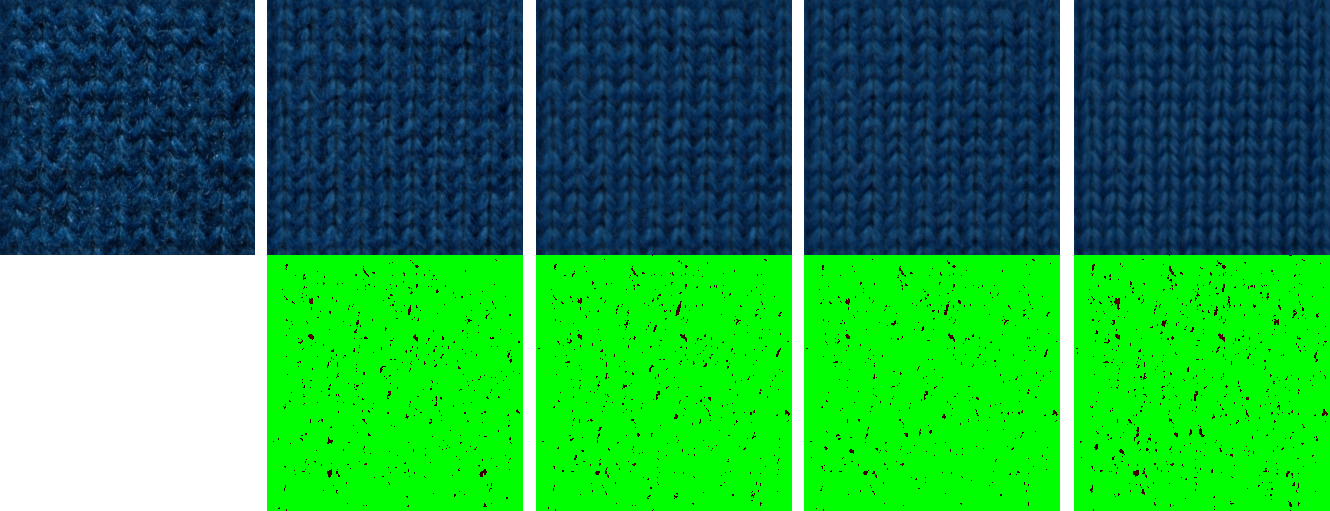
\includegraphics[width=1.0\textwidth]{figures/differ}
 \caption[Example of decompression errors ] {
 	{\bf Example of decompression errors }

	\textbf{First row} from the left to the right: ground truth, \textbf{32} components (MAE:2.17), \textbf{16} components (MAE:1.83), \textbf{8} components (MAE:2.21), \textbf{4} components (MAE:3.04). 
	\textbf{Second row}: the difference between the original and the decompressed images, \emph{red} color denotes how big the error, \emph{green} denotes that the error is absent or very small.}
 \label{fig:compression_example}
\end{figure}




 Figure \ref{fig:compression_example} shows that the decompression error is not significantly improved for $16$ or even $32$ components.
4 Components on the other hand result in a blurred image. This justifies our choice for 8 components.
 Haindl \cite{haindl} also shows that $8$ components is the optimal number of components for the PCA RF method, which is related to our method.



 
\begin{table}[h]
\begin{tabular}{|l|l|l|c|c|c|c|c|}
\hline
     & k                      & C                      & \begin{tabular}[c]{@{}c@{}}MAE\\  CIELab\end{tabular} & \begin{tabular}[c]{@{}c@{}}MAE \\ RGB\end{tabular} & \begin{tabular}[c]{@{}c@{}}RMSE\\  RGB\end{tabular} & \multicolumn{1}{l|}{Compression Ratio} & \begin{tabular}[c]{@{}c@{}}Parameters Size /\\  Storage Size (PNGs)\end{tabular} \\ \hline
wool & \multicolumn{1}{c|}{1} & \multicolumn{1}{c|}{8} & 2.14                                                  & 5.86                                               & 7.5                                                 & 1:23                                   & 53Mb / 20 Mb                                                                     \\ \hline
wool & 3                      & \multicolumn{1}{c|}{8} & 2.19                                                  & 6.83                                               & 8.68                                                & 1:70                                   & 18Mb / 5Mb                                                                       \\ \hline
wool & 3                      & 32                     & 2.22                                                  & 5.92                                               & 7.5                                                 & 1:17                                   & 70Mb / 25Mb                                                                      \\ \hline
\end{tabular}
\caption{ Evaluation of BTFs}
\label{table:mytable}
\end{table}


 Table \ref{table:mytable} provides the evaluation for the whole BTF space of the wool sample, i.e. for all possible camera and light directions.
 The MAE is also computed in RGB color space along with the Root Mean Square Error to measure the variance in the errors
 
 {\centering $RMSE = \sqrt{\frac{1}{N}\sum_{i=1}^{N}(y_i-\hat{y_i} )^2}$\\}

 RMSE gives large weights to big errors, thus we can evaluate if big errors are present \cite{rmse}.
 The bigger the RMSE the bigger the variance of the errors. We can see that in our case the RMSE is close to the MAE, which means that the variance of the errors is relatively small.
 
In the first row of the  Table \ref{table:mytable} where $k=1$ our method becomes equal to the PCA RF \cite{haindl} method.
Haindl \cite{haindl} has a MAE equal to $3.16$ in CIELAB color space for the same sample.
 Our method produces better result, i.e. $2.14$. 
 The second row shows that for  $k=3$ MAE stays practically the same. 
 However, the compression ratio improves by a factor of three.
 We can see that even for $32$ components decompression errors improve only insignificantly, but the compression ratio becomes worse.
 If we use $k>3$, more components would be necessary to reduce decompression errors.
 For intance, our method becomes equal to the PCA BTF \cite{haindl} method if $k=81$ (all camera directions). 
 In this case approximately $41$ components are necessary \cite{haindl}.
 
 Also, the LPCA BTF \cite{haindl} method uses $19$ components on average and has the MAE equal to $2.42$, while our method uses $8$ components.
 
 

\section{Real-time performance}
\label{section:eval_streaming}


We evaluate the rendering quality during the streaming and the real-time performance.
Figure \ref{fig:streamPreview} depicts intermediate images during the streaming.
We tested our approach on three materials: wool, impalla and corduroy.
The parameters for the compression are $k=3$ and $C=8$.

\begin{figure}[h]
 \centering
 \includegraphics[width=.87\textwidth]{figures/streampreview}
 \caption[Example of Progressive Streaming ] {
 	{\bf Example of Progressive Streaming}

	\textbf{From left to right}: \emph{1}, \emph{2}, \emph{4}, \emph{6}, \emph{8}  components rendered accordingly.
	}
 \label{fig:streamPreview}
\end{figure}
\label{chapter:implementation}



\begin{figure}[h]
 \centering
 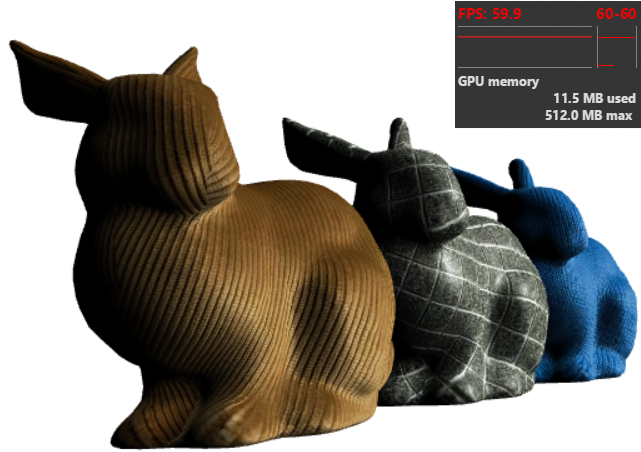
\includegraphics[width=.65\textwidth]{figures/3BTFs}
 \caption[Example of 3 BTFs rendered at the same time ] {
 	{\bf Example of 3 BTFs rendered at the same time }

	\textbf{From left to right}: corduroy, impalla and wool materials are rendered under dynamic light.
	}
 \label{fig:3BTFs}
\end{figure}
\label{chapter:implementation}

Rendering starts as soon as the first component transfers to the client side.
 The overall appearance of the the material is already visible even with the first component, which has an average size of about $0.7$ Mb.
With further components the overall quality of the image improves, i.e. specularities are increasing, small micro-structures become more visible and emphasized.
On a desktop computer with an NVIDIA GeForce GTX 480 graphics card 3 BTFs can be rendered at 60 frames per second.
Figure \ref{fig:3BTFs} shows an example of this.

On a mobile phone, Sony Xperia SL, 15 frames per second on average are achieved for one BTF at a time.


\section{Comparison with the Phong Shader}
\label{section:eval_streaming}

Figure \ref{fig:phongvsbtf} shows the tremendous difference between the BTF and a conventional 2-D texture in combination with the Phong shader.
Both images were taken under the same camera and light directions. The BTF introduces high varying specularities and the realistic depth in the images.
The Phong shader with the combination of the 2-D texture provides the impression that the material looks flat.
The BTF shows the correct inner-reflections, sub-surface scattering and shadows under varying light conditions.

\begin{figure}[hb]
 \centering
 \includegraphics[width=.73\textwidth]{figures/phongVsBTF}
 \caption[The Phong model in comparison to the BTF ] {
 	{\bf The Phong model in comparison to the BTF  }
	}
 \label{fig:phongvsbtf}
\end{figure}

